\documentclass[a4paper, 14pt]{article}

\usepackage[margin=3cm]{geometry}
\usepackage[utf8]{inputenc}
\usepackage[ngerman]{babel}
\usepackage[autostyle=true,german=quotes]{csquotes}
\usepackage{amsmath}
\usepackage{amssymb}
\usepackage{graphicx}
\usepackage{hyperref}
\usepackage{tikz}
\usepackage{multirow}
\usepackage{array}
\usetikzlibrary{
	calc
}

\author{Paul Brinkmeier}
\title{Cheatsheet für Einführung in Rechnernetze}

\begin{document}
	\maketitle
	\newpage
	\tableofcontents
	\newpage

	% \raggedright

	\section{Grundlegende Grundlagen}

	\paragraph{Rechnernetz}

	Ein Rechnernetz besteht aus Komponenten und Übertragungsmedien, die diese Komponenten miteinander verbinden.
	Übertragungsmedien realisieren die sogenannten Kommunikationslinks (Übertragungsstrecken) zwischen Komponenten.

	Komponenten sind beispielsweise Computer, Smartphones, Kühlschränke, Router.

	Medien sind beispielsweise Koaxialkabel, Kupferkabel, Glasfaser, Funk.

	\paragraph{Endsystem}

	Endsysteme (Hosts) führen verteilte Anwendungen aus.
	Diese benötigen ein Rechnernetz zur Kommunikation zwischen Anwendungsinstanzen.
	Beispiele für verteilte Anwendungen und Endsysteme: WhatsApp auf Smartphone, E-Mail auf Server, etc.

	\paragraph{Zwischensystem}

	Zwischensysteme leiten Daten im Netz weiter und führen i.d.R. keine verteilten Anwendungen aus.
	Beispiele für Zwischensysteme: Router, Switch.

	\paragraph{(Kommunikations-)Protokoll}

	Protokolle definieren Regeln und Formate für die Kommunikation zwischen zwei oder mehreren Computern sowie die beim Senden und Empfangen von Daten bzw. bei Ereignissen auszuführenden Aktionen.

	\paragraph{(Daten-)Pakete}

	Die von Anwendungen zu sendenden Daten können in kleinere Teile gegliedert werden.
	Diese werden als (Daten-)Pakete bezeichnet.
	Pakete sind aufgebaut aus Metadaten und Nutzdaten.
	Metadaten sind nur für die Abwicklung des Protokolls erforderlich; Nutzdaten sind die eigentlichen für die Anwendung wichtigen Daten.
	I.d.R. werden Pakete in Rechnernetzen unabhängig voneinander bearbeitet.

	\paragraph{Datenrate (Übertragungsrate)}

	Die Datenrate bezeichnet die Geschwindigkeit, mit der Daten zwischen zwei Komponenten übertragen wird.
	Sie wird in bit/s gemessen.
	Größenordnungen: K, M, G, T, etc. \emph{nicht} Ki, Mi, Gi, Ti!

	\subsection{Netzkern und Netzrand}

	\paragraph{Netzkern}

	Der Netzkern besteht aus den Netzen untereinander verbunderer Internet Service Provider (ISPs).
	Er beschäftigt sich vor allem mit der Weiterleitung von Paketen.
	Der Netzkern ist sozusagen das \enquote{Betriebssystem} des Internets.

	\paragraph{Netzrand}

	Der Netzrand besteht aus den Netzen von Endandwendern, bspw. Heimnetze, Firmennetze und Datenzentren.
	Er beherbergt die \enquote{Anwendungen} des Internets.

	\subsection{\enquote{Provider} im Internet}

	\paragraph{Internet-Service-Provider (ISP)}

	ISPs binden Konsumenten an das Internet an.
	Dazu gehören oft tausende Kunden und auch Unternehmen.
	Bspw. Unitymedia, Telekom, 1\&1.

	Verschiedene Größenordnungen: Tier-1-ISP, Regionaler ISP, Zugangs-ISP.

	\subparagraph{Warum hierarchisch?}

	Vernetzung aller $n$ Zugangs-ISPs Verbindungen $\in O(n^2)$ $\leadsto$ skaliert nicht.

	\paragraph{Internet-Exchange-Point (IXP)}

	IXPs sorgen für Datenaustausch zwischen größeren ISPs.
	Es gibt weltweit ca. 400 IXPs.

	\paragraph{Content-Provider}

	Content-Provider erzeugen und stellen Inhalte bereit.
	Sie wollen diese so nah wie möglich an den Netzrand ($\leadsto$ zu den Kunden) bringen.
	Bspw. Google, Netflix, Amazon.

	\subsection{Modellierung}

	\paragraph{Modell}

	Ein Modell ist ein vereinfachtes Abbild der Wirklichkeit.
	Man setzt Modelle ein, um die wesentlichen Aspekte eines Systems darzustellen.
	Die innere Struktur des Systems wird abstrahiert; man modelliert die Interaktion mit dem System (Black-Box).

	\subsubsection{Grundmodell der Kommunikation}

	\begin{itemize}
		\item Sender und Empfänger (je einer oder mehrere).
		\item Abstraktes Medium.
	\end{itemize}

	\paragraph{Abstraktes Medium}
	
	Das Medium verbindet Sender und Empfänger über eine räumliche Distanz.
	Es stellt damit einen (Kommunikations-)Dienst zur Verfügung.
	Den Übergang von Sender/Empfänger zum Medium nennt man Schnittstelle.

	Ein abstraktes Medium trifft keinerlei Aussage über seine konkrete (physische) Umsetzung.

	\subsubsection{Dienstesicht}

	\paragraph{Dienstesicht}

	Betrachtung eines Rechnernetzes als Black-Box.
	Das RN erbringt einen Dienst für seine Nutzer.

	Das RN entspricht hier dem abstrakten Medium.

	\paragraph{Dienst}

	Ein Dienst bündelt zusammengehörige Funktionen und stellt diese einem Nutzer (Dienstnehmer) zur Verfügung.
	Einzelen Teile eines Dienstes können unabhängig voneinander in Anspruch genommen werden.

	Ein \emph{Dienstzugangspunkt} (Service Access Point, SAP) stellt die Schnittstelle zu einem Dienst dar.

	\emph{Dienstnehmer} nehmen eine Dienst in Anspruch.

	\emph{Dienstgeber} (Diensterbringer) stellen einen Dienst zur Verfügung.

	\emph{Dienstprimitive} beschreiben die Interaktionen zwischen Dienstnehmer und Dienstgeber.

	Die \emph{Beschreibung eines Dienstes} reflektiert das Verhalten an den Dienstzugangspunkten zum Dienstgeber.

	\begin{figure}
		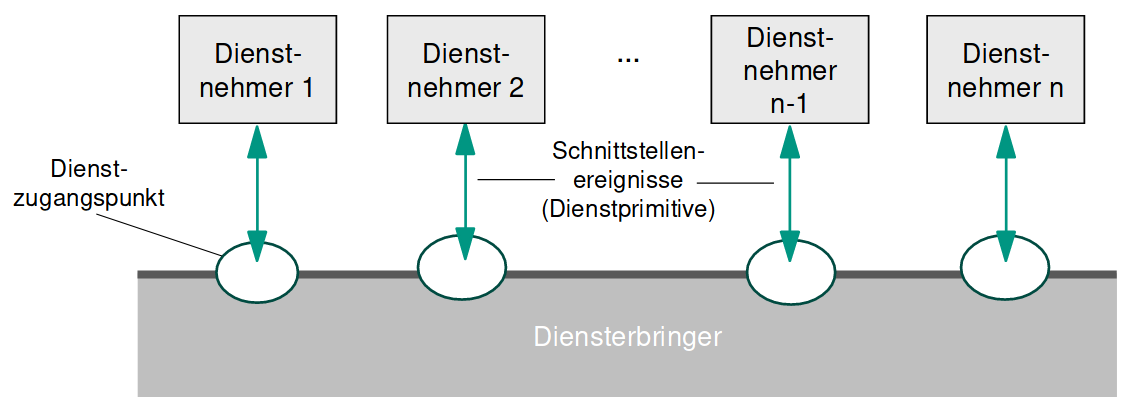
\includegraphics[width=\textwidth]{images/02-services.png}
		\caption{Dienstesicht}
	\end{figure}

	\paragraph{Dienstprimitive}

	\begin{itemize}
		\item \emph{Request} (req) --- Dienstnehmer 1 (DN1) beauftragt Dienstgeber.
		\item \emph{Indication} (ind) --- Dienstgeber benachrichtigt Dienstnehmer 2 (DN2) über Auftrag.
		\item \emph{Response} (res) --- DN2 beantwortet Auftrag.
		\item \emph{Confirmation} (cnd) --- Dienstgeber benachrichtigt DN1 über Abschluss.
	\end{itemize}

	\begin{figure}
		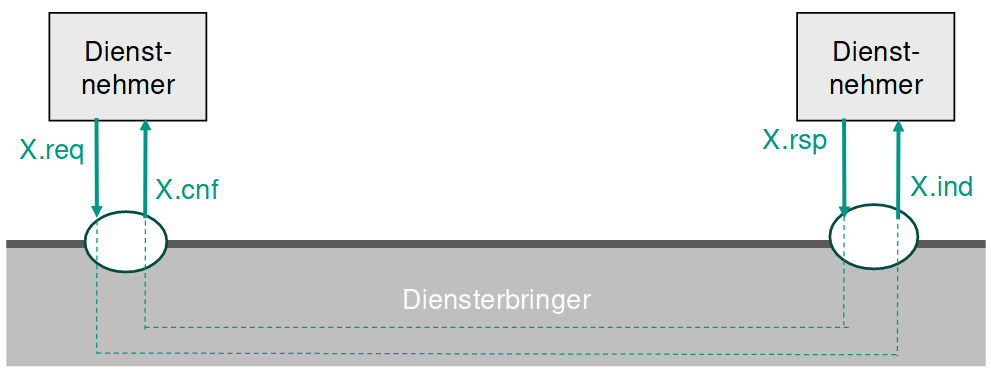
\includegraphics[width=\textwidth]{images/02-primitives.png}
		\caption{Dienstprimitive}
	\end{figure}

	\paragraph{Formen von Diensten}

	\begin{itemize}
		\item Unbestätigter Dienst --- Request (DN1), Indication (DN2).
		\item Bestätigter Dienst --- Request (DN1), Indication (DN2), Response (DN2), Confirmation (DN1).
	\end{itemize}

	\begin{figure}
		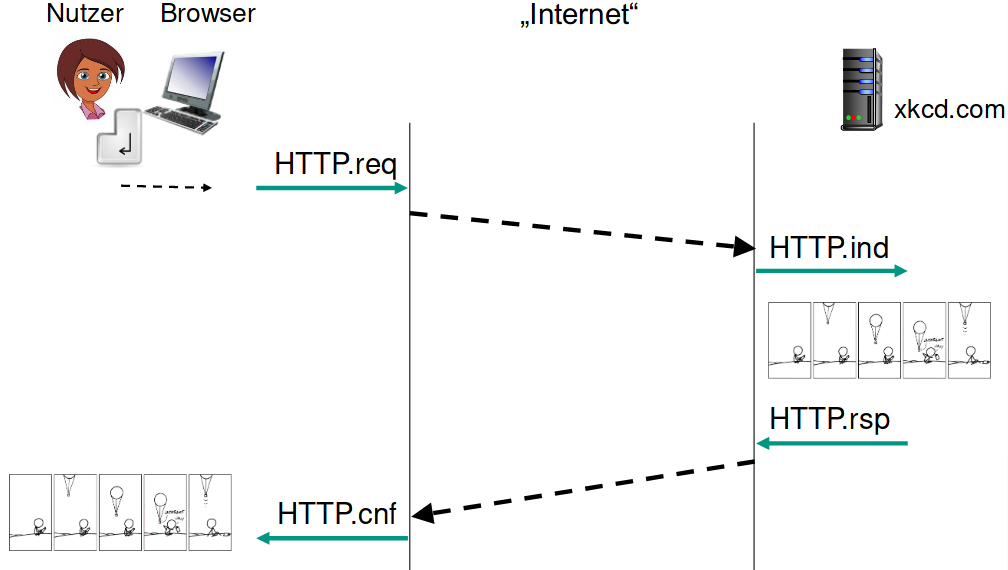
\includegraphics[width=\textwidth]{images/02-http-example.png}
		\caption{Beispiel für einen bestätigten Dienst: HTTP}
	\end{figure}

	\subsection{Zuverlässiger Dienst}

	\paragraph{Zuverlässiger Dienst}

	Bei einem zuverlässigen Dienst gilt am Dienstzugangspunkt des Empfängers folgendes:

	\begin{itemize}
		\item Alle empfangenen Daten sind korrekt.
		\item Alle vom Sender zu empfangenden Daten werden vollständig und in der richtigen Reiehnfolge empfangen.
		\item Es werden keine Duplikate empfangen.
		\item Es werden keine Phantom-Daten empfangen.
	\end{itemize}

	\textbf{Merke}: Zuverlässiger Dienst (ZD) $\neq$ Bestätigter Dienst (BD).
	Es gilt eher BD $\subset$ ZD.
	Bestätigungen sind nur \enquote{ein Baustein} zuverlässiger Dienste.

	\subsection{Schichten}

	\paragraph{Schicht}

	Eine Schicht bündelt zusammengehörige Funktionalitäten, die sich von denen anderer Schichten unterscheiden.
	Schichten sind hierarchisch angeordnet.
	An ihrer Schnittstelle stellt eine Schicht Dienste für die nächst-\enquote{höhere} Schicht bereit und nutzt Dienste der nächst-\enquote{unteren} Schicht.
	Die technische Umsetzung einer Schicht ist an dieser Schnittstelle nicht sichtbar.
	Zur Erbringung ihrere Dienste nutzt eine Schicht die Dienste der darunter liegenden Schicht.

	Protokolle sind innerhalb einer Schicht lokalisiert.

	\begin{figure}
		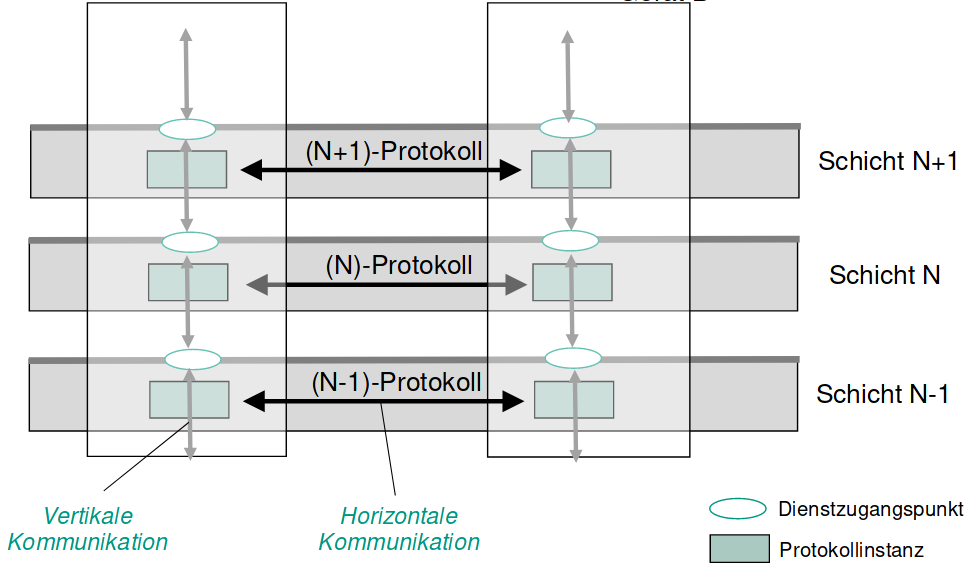
\includegraphics[width=\textwidth]{images/02-layers.png}
		\caption{Protokolle, Dienste, Schichten}
	\end{figure}

	\paragraph{Horizontale Kommunikation}

	Horizontale Kommunikation findet innerhalb einer Schicht zwischen Sender und Empfänger statt.
	Die Protokollinstanzen der Schicht (auf den jeweiligen Geräten) tauschen Daten untereinander aus, um den geforderten Dienst zu erbringen.

	\paragraph{Vertikale Kommunikation}

	Vertikale Kommunikation findet zwischen zwei Schichten innerhalb eines Gerätes statt.
	Protokollinstanz der Schicht $N$ nimmt Dienste der Schicht $N - 1$ in Anspruch oder reichen Daten an Schicht $N + 1$ weiter.

	\subsubsection{Fünf-Schichten-Referenzmodell}

	\begin{figure}
		\begin{center}
			\begin{tikzpicture}[
	>=latex
]
	\node(layers)[inner sep=0]{\Large \begin{tabular}{| c |}
		\hline
		Anwendungsschicht \\
		\hline
		Transportschicht \\
		\hline
		Vermittlungsschicht \\
		\hline
		Sicherungsschicht \\
		\hline
		Physische Schicht \\
		\hline
	\end{tabular}};

	\coordinate (T) at ($(layers.north east) + (1cm, 0)$);
	\coordinate (B) at ($(layers.south east) + (1cm, 0)$);

	\draw[->] (B) -- (T);

	\node[anchor=west] at (T) {Abstraktion hoch};
	\node[anchor=west] at (B) {Abstraktion niedrig};
\end{tikzpicture}

		\end{center}
		\caption{Referenzmodell mit fünf Schichten}
	\end{figure}

	\paragraph{Physische Schicht}

	Zwei direkt über ein Übertragungsmedium beschränkter Länge verbundene Geräte können unstrukturierte Bitfolgen austauschen.
	Eigenschaften dieser Schicht sind:

	\begin{itemize}
		\item Stellt unzuverlässigen Dienst für (Sicherungsschicht) bereit.
		\item Bits werden nicht gepuffert.
		\item Stark Hardwareabhängig (\enquote{LAN-Kabel}, Glasfaser, WLAN, etc.).
		\item Bei der Übertragung können Störungen auftreten (Paradebeispiel: WLAN).
	\end{itemize}

	\paragraph{Sicherungsschicht}

	Auf dieser Schicht werden zwischen physisch benachbarten Systemen Daten Paketweise (sog. \emph{Rahmen}) übertragen.
	Eigenschaften dieser Schicht sind:

	\begin{itemize}
		\item Ermöglicht Adressierung benachbarter Geräte.
		\item Stellt unzuverlässige und zuverlässige Dienste (Erkennung von Fehlern der physischen Schicht) bereit.
		\item Puffert Daten sowohl beim Sender als auch beim Empfänger.
		\item Abstrahiert physisches Medium.
	\end{itemize}

	\paragraph{Vermittlungsschicht}

	Diese Schicht ermöglicht den Austausch von Daten zwischen (nicht unbedingt) benachbarten Systemen über Zwischensysteme (\emph{Ende-zu-Ende}).
	Pakete nennt man hier typischerweise \emph{Datagramme}.
	Eigenschaften dieser Schicht sind:

	\begin{itemize}
		\item Universale Adressierung von Endsystemen (bspw. IP-Adressen).
		\item Stellt unzuverlässige und zuverlässige Dienste bereit.
		\item Datagramme können in Zwischensystemen gepuffert werden.
		\item Ein Datagramm wird in einem oder mehreren Rahmen der Sicherungsschicht übertragen.
	\end{itemize}

	\paragraph{Transportschicht}

	In dieser Schicht ist die Kommunikation zwischen Anwendungsprozessen auf den Endsystemen gekapselt (\emph{Nutzer-zu-Nutzer}).
	Pakete nennt man hier typischerweise \emph{Datagramme} oder \emph{Segmente}.
	Eigenschaften dieser Schicht sind:

	\begin{itemize}
		\item Adressierung von Anwendungsprozessen auf Endsystemen (\emph{Ports}).
		\item Stellt unzuverlässige (bspw. UDP) und zuverlässige (bspw. TCP) Dienste bereit.
		\item Segmente/Datagramme werden in Endsystemen gepuffert.
		\item Ein Segment/Datagramm wird in einem oder mehreren Datagrammen der Vermittlungsschicht übertragen.
	\end{itemize}

	\paragraph{Anwendungsschicht}

	Über diese Schicht tauschen Anwendungen untereinander \emph{Nachrichten} (bspw. HTTP-Response) aus.
	Je nach Anwendung werden hier zuverlässige oder unzuverlässige Dienste der Transportschicht genutzt.

	\subsubsection{TCP/IP-Referenzmodell}

	Im Internet am weitesten verbreitet (quasi alleinstehend) ist das TCP/IP-Modell.
	Dieses definiert in \href{https://tools.ietf.org/html/rfc1122}{RFC 1122} vier Schichten:

	\begin{center}
		\Large
		\begin{tabular}{| c |}
			\hline
			Anwendungsschicht \\
			\hline
			Transportschicht \\
			\hline
			Internetschicht \\
			\hline
			Netzzugang \\
			\hline
		\end{tabular}
	\end{center}

	Die Internetschicht entspricht der Vermittlungsschicht; Netzzugang kombiniert phyisische und Sicherungsschicht.
	
	\subsubsection{OSI-Referenzmodell}

	Das von der ISO standardisierte OSI-Modell (Open Systems Interconnection Model) definiert sieben Schichten:

	\begin{center}
		\Large
		\begin{tabular}{| c | c}
			\cline{1-1}
			Anwendungsschicht & \multirow{3}{*}{\normalsize Anwendungsorientierte Schichten} \\
			\cline{1-1}
			Darstellungsschicht & \\
			\cline{1-1}
			Sitzungsschicht & \\
			\hline
			Transportschicht & \multirow{4}{*}{\normalsize Transportorientierte Schichten} \\
			\cline{1-1}
			Vermittlungsschicht & \\
			\cline{1-1}
			Sicherungsschicht & \\
			\cline{1-1}
			Physische Schicht & \\
			\cline{1-1}
		\end{tabular}
	\end{center}

	\paragraph{Transportorientierte Schichten}

	Transportorientierte Schichten befassen sich mit der Übertragung von Daten zwischen Anwendungen.
	Die Semantik der übertragenen Daten spielt dabei keine Rolle.

	\paragraph{Anwendungsorientierte Schichten}

	Hier werden Anwendungsbezogene Protokolle abgewickelt.
	Die Semantik der übertragenen Daten ist wichtig.

	\begin{itemize}
		\item \emph{Sitzungsschicht} --- Bietet Nichtunterbrechbarkeit von Kommunikationsbeziehungen.
		\item \emph{Darstellungsschicht} --- Vereinheitlicht Darstellung der Daten über heterogene Systeme hinweg (bspw. Litte- vs. Big-Endian).
		\item \emph{Anwendungsschicht} --- Austausch von anwendungsspezifischen Daten.
	\end{itemize}

	\subsubsection{TCP/IP vs. OSI}

	\begin{itemize}
		\item Netzzugang $\Leftrightarrow$ OSI-Schichten 1 und 2 (physische Schicht, Sicherungsschicht).
		\item Schichten 3 und 4 (Vermittlungsschicht, Transportschicht) sind identisch.
		\item Anwendungsschicht $\Leftrightarrow$ OSI-Schichten 5 bis 7 (Sitzungs-, Darstellungs- und Anwendungsschicht).
	\end{itemize}

	Beim TCP/IP-Referenzmodell wird weniger granular zwischen den Schichten unterschieden.
	Das liegt daran, dass dieses Modell sich eher mit der Zeit aus Prototypen entwickelt hat, als dass es entworfen worden wäre.

	\section{Physische Schicht}

	\subsection{Abstraktes Modell nach Shannon}

	Allgemeine Erkenntnisse, die für alle Arten der Datenübertragung gelten (bspw. Morsen, Telefon, WhatsApp).
	Sender, Empfänger und Kanal sind hier Komponenten der physischen Schicht.

	\paragraph{Informationsquelle}

	Liefert Nachricht in Form einer Bitfolge in vorgegebenem Takt an den Sender.

	\paragraph{Sender}

	Wandelt Nachricht in Signal um und sendet dieses auf den Kanal.

	\paragraph{Kanal}

	Das Medium wird hier als (Übertragungs-)Kanal bezeichnet.
	Eine \emph{Störquelle} kann das Signal beeinflussen.

	\paragraph{Empfänger}

	Rekonstruiert Nachricht aus dem Empfangssignal und übergibt sie der \emph{Informationssenke}.

	\begin{figure}
		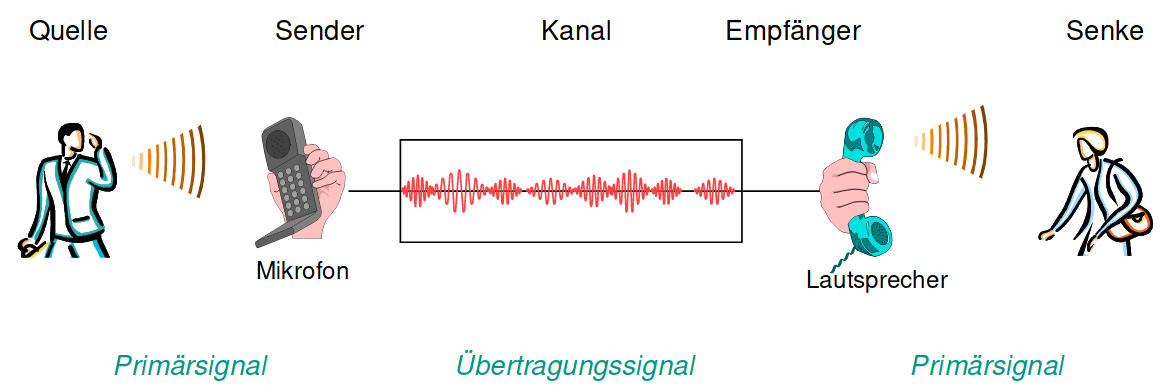
\includegraphics[width=\textwidth]{images/03-shannon-telephone.png}
		\caption{Abstraktes Modell nach Shannon am Beispiel der Telefonie}
	\end{figure}

	\subsection{Medium}

	Das Medium (der Kanal) verbindet auf der physischen Schicht physisch benachbarte Geräte.
	Die Distanz zwischen den Geräten muss überbrückbar sein.
	Um die überbrückbare Distanz zu erhöhen, kommen sogenannte Repeater zum Einsatz, die das Signal verstärken.
	Netze können verschiedenste Medien verwenden; beispielsweise WLAN, UMTS, Kupferkabel oder Glasfaser.

	\subsection{Signal}

	Mit einem Signal können Informationen übertragen werden.
	Formal ist ein Signal eine Funktion $s : T \to V$.
	Zum Zeitpunkt $t$ nimmt das Signal den (Signal-)Wert $s(t)$ ein.

	Signale werden als zeit- und wert-kontinuierlich oder -diskret klassifiziert.
	Diskret heißt hierbei salopp gesagt $T\text{ bzw. }V = \mathbb{Z}$; kontinuierlich heißt $T\text{ bzw. }V = \mathbb{R}$.

	\begin{figure}
		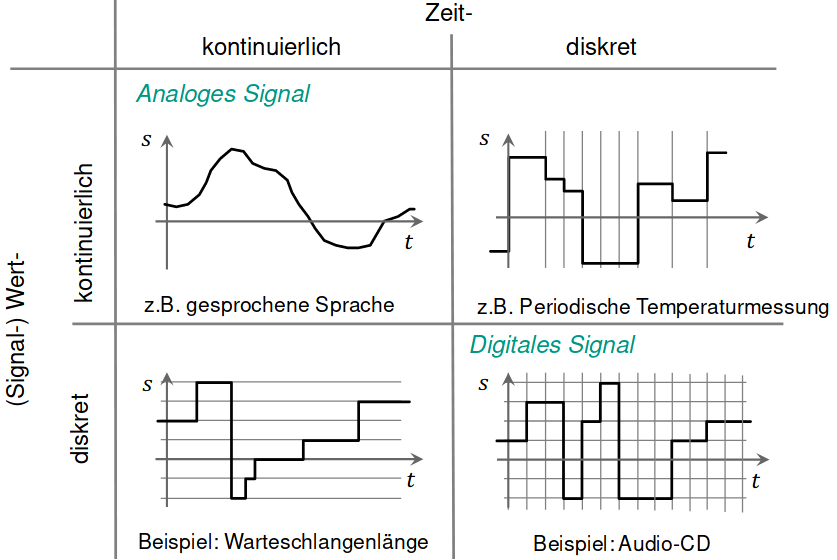
\includegraphics[width=\textwidth]{images/03-signal-classification.png}
		\caption{Klassifizierung von Signalen}
	\end{figure}

	\subsubsection{Digitales Signal}

	Ein digitales Signal ist sowohl zeit- als auch wert-diskret.

	\paragraph{Isochrones digitales Signal}

	Bei einem isochronen digitalen Signal erfolgen Wechsel des Signalwertes nur zum Schritttakt.

	\subsubsection{Analoges Signal}

	Ein analoges Signal ist sowohl zeit- als auch wert-kontinuierlich.

	\paragraph{Periodische Signale}

	Periodische Signale haben eine \emph{Periodendauer} $T$, d.h. der Signalwert wiederholte sich alle $T$ Zeiteinheiten:

	\begin{equation*}
		\forall n \in \mathbb{N} : s(t) = s(t + n \times T)
	\end{equation*}

	Die \emph{Frequenz} $f$ eines periodischen Signals ist definiert als $f = \frac{1}{T}$.

	Merke (aus HM): eine periodische Funktion lässt sich als Summe von Sinus- und Kosinusfunktionen schrieben (Fourier-Reihe).

	Wichtige Parameter der Sinus- und Kosinusfunktionen sind deren Amplitude, Frequenz und Phase.

	\begin{figure}
		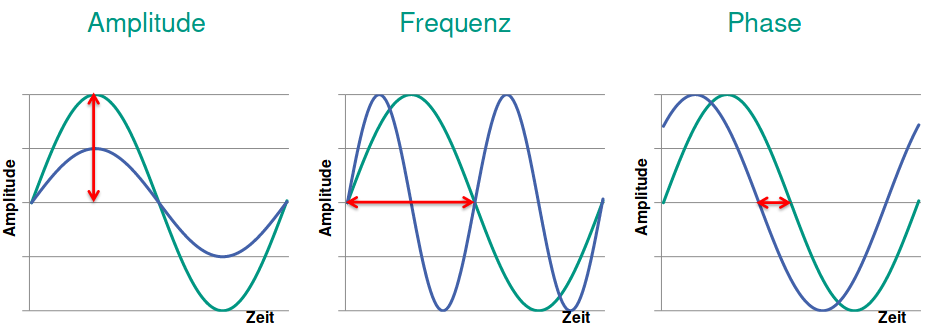
\includegraphics[width=\textwidth]{images/03-trig.png}
		\caption{Parameter trigonometrischer Funktionen}
	\end{figure}

	\subsection{Shannonsche Kanalkapazität}

	\begin{align*}
		C &= B \times \log_2\left(1 + \frac{S}{N}\right)\text{bit} \\
		\frac{S}{N} &= 10 \times \log_{10}\frac{\text{\tiny Signalenergie}}{\text{\tiny Störenergie}}
	\end{align*}

	\begin{itemize}
		\item $C$: Kanalkapazität in bit/s.
		\item $B$: Bandbreite in Hz.
		\item $\frac{S}{N}$: Verhältnis Signal- zu Störenergie.
	\end{itemize}

	Die Kanalkapazität beschreibt die maximale Datenrate, die aufgrund der gegebenen Randbedingungen über einen längeren Zeitraum hinweg aufrecht erhalten werden kann.

	\paragraph{Beispiel:}

	Gegeben sei die Bandbreite $B = 4\text{kHz}$ und das Verhältnis der Signal- zur Störenergie $30\text{dB} \Rightarrow \frac{S}{N} = 10^3$. Also:

	\begin{equation*}
		C = 4\text{kHz} \times \log_2\left(1 + 10^3\right)\text{bit} \approx 40\text{kbit/s}
	\end{equation*}

	\subsection{Modulation und Leitungscodierung}

	Der Sender erhält von der Informationsquelle die Nachricht in Form einer Bitfolge und erzeugt daraus ein phyisisches Signal.
	Innerhalb des Senders agieren der Leitungscodierer und der Modulator.

	\paragraph{Leitungscodierer}

	Der Leitungscodierer bereitet der Bitstrom für die Übertragung vor (bspw. fehlerkorrigierende Codes).

	\paragraph{Modulator}

	Der Modulator bildet aus der codierten Nachricht die physischen Signale.

	\subsection{Modulation}

	Durch Modulation (Veränderung) sinusförmiger Trägersignale wird ein zu übertragendes Nutzsignal für die physische Übertragung ausbereitet.
	Ein zu sendendes digitales Signal wird zur Übertragung in ein analoges überführt.

	\subsubsection{Amplitudenumtastung}

	Hierbei wird die Amplitude des Trägersignals verändert.
	In ihrer einfachsten Form besteht Amplitudenumtastung aus dem Ein- und Ausschalten (zur Übertragung einer 1 bzw. einer 0) des Trägersignals.

	Amplitudenumtastung ist leicht zu implementieren, benötigt wenig Bandbreite, ist aber anfällig für Störungen.

	\subsubsection{Frequenzumtastung}

	Hierbei wird jedem möglichen Signalwert (bspw. 0 und 1) eine Frequenz zugewiesen.

	Frequenzumtastung benötigt eine größere Bandbreite als Amplitudenumtastung.

	\subsubsection{Phasenumtastung}

	Bei Phasenumtastung wird jedem möglichen Signalwert eine bestimmten Phase der Sinusfunktion zugeordnet.

	Phasenumtastung ist zwar komplex in der Umsetzung, jedoch relativ störungssicher.

	\subsection{Leitungscodierung}

	\subsubsection{Codierung}

	Seien $A$ und $B$ endliche Alphabete.
	Eine Codierung ist eine injektive Abbildung $c : A^+ \to B^+$.
	Man nennt $A$ das \emph{Quellenalphabet} und $B$ das \emph{Codealphabet} von $c$.

	\paragraph{Beispiel Morsecode}

	\begin{align*}
		A &= \{\text{A}, ..., \text{Z}, 0, ..., 9, \text{\emph{Punkt}}, \text{\emph{Komma}}, \text{?}\} \\
		B &= \{\bullet-, ..., --\bullet\bullet, ...\} \\
		\\
		c(\text{A}) &= \bullet- \\
		c(\text{Z}) &= --\bullet\bullet \\
		c(\text{SAAAS}) &= \bullet\bullet\bullet\bullet-\bullet-\bullet-\bullet\bullet\bullet
	\end{align*}

	\paragraph{Code}

	Sei $c$ eine Codierung.
	Der von $c$ erzeugte Code ist die Menge

	\begin{equation*}
		C := c(A) = \{ c(z) : z \in A \}
	\end{equation*}

	$c(z) \in B$ nennt man das Codewort eines Zeichens $w \in A$.

	\subsubsection{Mehrwertige Digitalsignale}

	Ein binäres Digitalsignal ist zeit- und wert-diskret.
	Es kann nur zwei Werte annehmen: 0 und 1.
	Ein mehrwertiges Digitalsignal ist zeit- und wert-diskret und kann mehr als zwei Werte annehmen.
	Beispielsweise kann ein quaternäres Signal 4 verschiedene Signalwerte annehmen und damit $\log_2{}4 = 2$ Bit pro Schrittdauer darstellen.

	\subsubsection{Baudrate}

	\paragraph{Übertragungsgeschwindigkeit}
	
	Die Übertragungsgeschwindigkeit (Datenrate) bezeichnet die Anzahl der übertragenen Bits in einer Schrittdauer in bit/s.

	\paragraph{Schrittgeschwindigkeit}

	Die Schrittgeschwindigkeit (Baudrate) bezeichnet die Anzahl der Signalwertwechsel innerhalb eines Schrittes in baud ($=$ bit/s).

	\begin{figure}
		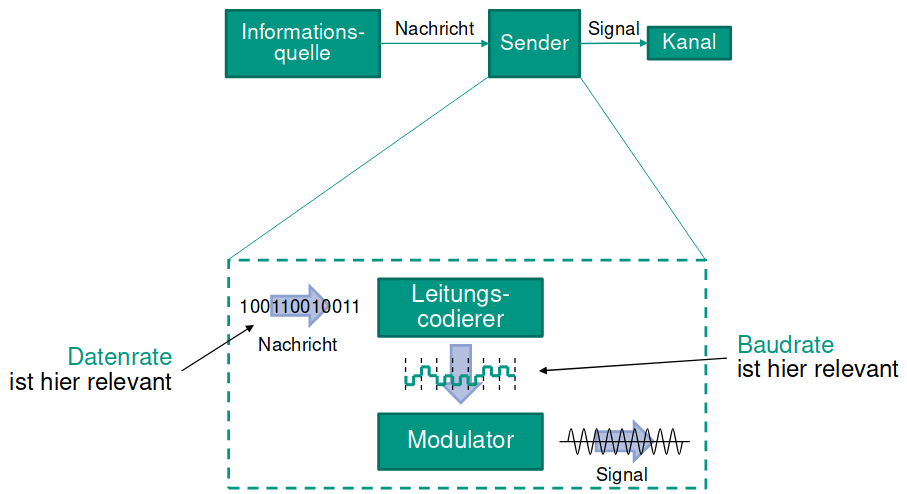
\includegraphics[width=\textwidth]{images/03-baudrate-datarate.png}
		\caption{Baudrate und Datenrate}
	\end{figure}

	\subsection{Leitungscodes}

	Ziele von Leitungscodes sind:

	\paragraph{Taktrückgewinnung}

	Sender um Empfänger verfügen i.d.R. über keinen gemeinsamen Takt.
	Der Empfänger sollte aus den Signalwerten den Takt rekonstruieren können.
	Dies sollte unabhängig vom Inhalt der übertragenen Daten möglich sein.

	\paragraph{Niedrige Baudrate}

	Anzahl der Signalwertwechsel pro Schrittdauer gering halten.

	\paragraph{Geringe Komplexität}

	Kosten, Baugröße, Energieaufnahme, etc. sollten gering sein.

	% TODO: Gleichstromzeug

	\subsubsection{NRZ}

	Bei NRZ (Non-Return to Zero) werden die Symbolwerte durch die Signalwerte bestimmt.
	Eine 1 (0) in der Nachricht wird als hoher (niedriger) Pegel über ein gesamtes Taktintervall codiert.
	Signalwertwechsel erfolgen an den Taktgrenzen; die Erkennung des Signals erfolgt direkt durch auslesen des Pegels.

	\begin{figure}
		\begin{center}
			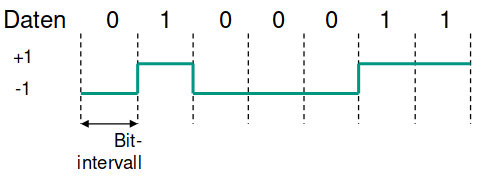
\includegraphics[width=0.6\textwidth]{images/03-nrz.png}
		\end{center}
		\caption{NRZ-Codierung des Wortes 010001}
	\end{figure}

	Die Baudrate ist bei NRZ recht niedrig (Signalwertwechsel nur bei 0-1- bzw. 1-0-Übergängen).
	Taktrückgewinnung ist bei längeren 0- oder 1-Folgen jedoch nicht möglich.

	\subsubsection{Manchester}

	Der Manchester-Code ist ein sogenannter Biphasen-Code: Symbolwerte werden durch Phasensprünge bestimmt.
	Eine 1 (0) in der Nachricht wird als Signalübergang vom hohen Pegel zum niedrigen Pegel (vom niedrigen zum hohen Pegel) in der Intervallmitte codiert.
	Bei 0-Folgen oder 1-Folgen müssen also \enquote{Hilfswechsel} eingefügt werden, um mehrfache Phasensprünge in derselben Richtung zu ermöglichen.

	\begin{figure}
		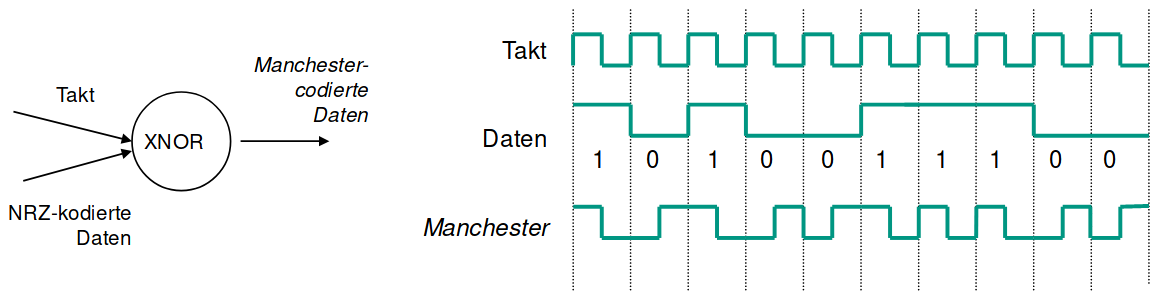
\includegraphics[width=\textwidth]{images/03-manchester.png}
		\caption{Manchester-Codierung des Wortes 1010011100}
	\end{figure}

	Taktrückgewinnung lässt sich beim Manchester-Code recht einfach umsetzen, da mindestens ein Signalwertwechsel pro Taktintervall auftritt.
	Die Baudrate ist jedoch sehr hoch; bei 0-Folgen oder 1-Folgen ist sie doppelt so hoch wie die Datenrate.
	Die Implementierung des Manchester-Codes ist einfach; er ist die XNOR-Verknüpfung der Daten und des Taktes.

	\subsubsection{AMI}

	AMI (Alternate Mark Inversion) nutzt einen ternären Code mit den möglichen Werten -1, 0 und 1.
	Eine 0 in der Nachricht wird als 0 über ein gesamtes Taktintervall codiert.
	Eine 1 wird abwechselnd als -1 und 1 über ein gesamtes Taktintervall codiert.

	\begin{figure}
		\begin{center}
			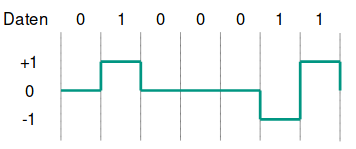
\includegraphics[width=0.6\textwidth]{images/03-ami.png}
		\end{center}
		\caption{AMI-Codierung des Wortes 0100011}
	\end{figure}

	Taktrückgewinnung ist bei AMI bei langen 0-Folgen nicht möglich.
	Die Baudrate ist bei AMI einigermaßen niedrig (Signalwertwechsel an 0-1, 1-0 und 1-1-Übergängen aber nicht bei 0-0).

	\subsection{Störquellen}

	Wie bereits erwähnt kann eine Störquelle das Signal auf einem Kanal beeinflussen.
	Wichtige Beeinträchtigungen sind:

	\begin{itemize}
		\item \emph{Dämpfung} (Attenuation)
		\item \emph{Verzögerung} (Delay Distortion)
		\item \emph{Rauschen} (Noise)
	\end{itemize}

	\subsubsection{Dämpfung}

	Die Stärke eines Signales sinkt mit zunehmender Distanz.
	Beschrieben in dB/m.
	Beim Empfänger muss die Signalstärke noch groß genug sein, um das Signal überhaupt zu erkennen und größer als das Rauschen.
	Dafür können Verstärker oder Repeater eingsetzt werden.

	\subsubsection{Verzerrung}

	Durch die Verzögerung der Signalausbreitung entsteht Verzögerungsverzerrung.
	Diese variiert mit der Frequenz.
	Da unterschiedliche Frequenzen den Empfänger zu verschiedenen Zeiten erreichen können, kann es zu Phasenverschiebung zwischen den Frequenzen.
	Aufeinanderfolgende Bits können dadurch überlappen.
	Dies nennt man \emph{Intersymbol-Interferenz}.

	\begin{figure}
		\begin{center}
			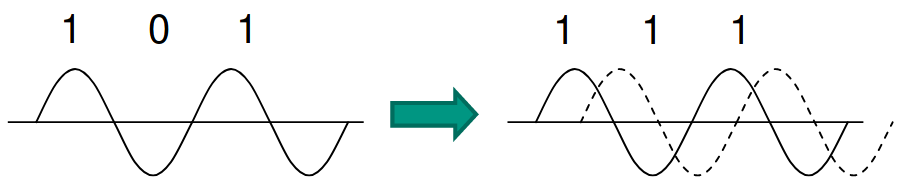
\includegraphics[width=0.6\textwidth]{images/03-intersymbol-interference.png}
		\end{center}
		\caption{Verzögerungsverzerrung (Intersymbol-Interferenz)}
	\end{figure}

	\subsubsection{Rauschen}

	\paragraph{Thermisches Rauschen}

	Thermisches Rauschen ist eine Funktion der Temperatur.
	Es ist gleich verteilt über Frequenzen hinweg (\enquote{weißes Rauschen}) und kann nicht eliminiert werden.
	Es bestimmt damit die maximales Leistungsfähigkeit.

	\paragraph{Modulationsrauschen}

	Zwei Frequenzen überlagern sich.

	\paragraph{Impulsrauschen}

	Impulsrauschen wird hervorgerufen von elektromagnetischen Störungen wie bspw. Blitzen.
	Es macht sich bemerkbar durch unregelmäßige Ausschläge und Geräuschspitzen kurzer Dauer und hoher Amplitude.

	\begin{figure}
		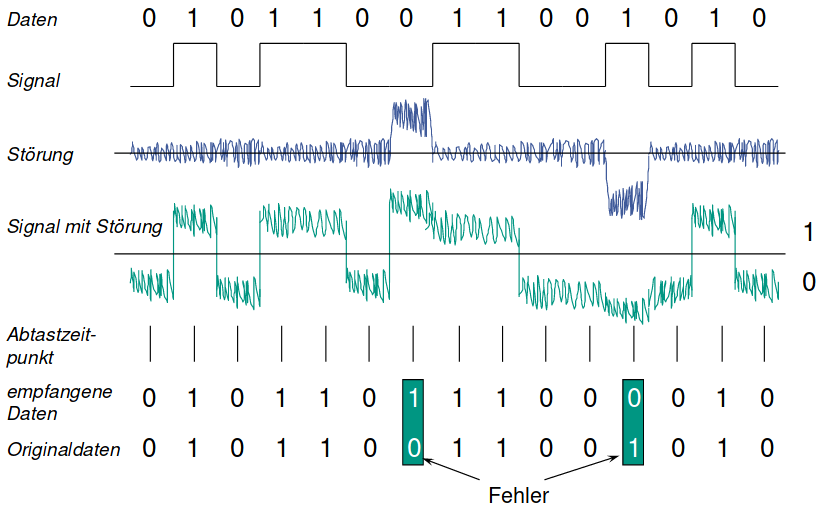
\includegraphics[width=\textwidth]{images/03-error.png}
		\caption{Auswirkung von Störungen}
	\end{figure}

	\section{Sicherungsschicht}

	\section{Vermittlungsschicht}

	\section{Transportschicht}

	\section{Anwendungsschicht}

	\section{Netzssicherheit}

	\section{Klausuraufgaben}
\end{document}
